\section{Kết quả và phân tích}
\label{sec:ket-qua-va-phan-tich}

\subsection{Kết quả trên dữ liệu đầy đủ (0\% thiếu)}
\label{sec:ket-qua-du-lieu-day-du}

\begin{table}[H]
\centering
\caption{Hiệu năng của tất cả mô hình và baseline trên tập test, không giả lập thiếu dữ
liệu (0\%).}
\label{tab:ket-qua-day-du}
\begin{tabular}{@{}lcccc@{}}
\toprule
\textbf{Mô hình} & \textbf{Macro F1} & \textbf{PR-AUC} & \textbf{Precision} & \textbf{Recall} \\
\midrule
Lớp đa số & \TODO{} & \TODO{} & \TODO{} & \TODO{} \\
Persistence & \TODO{} & \TODO{} & \TODO{} & \TODO{} \\
Ngưỡng nhiệt độ & \TODO{} & \TODO{} & \TODO{} & \TODO{} \\
Logistic Regression & \TODO{} & \TODO{} & \TODO{} & \TODO{} \\
k-NN & \TODO{} & \TODO{} & \TODO{} & \TODO{} \\
XGBoost (LiteStatTemp) & \TODO{} & \TODO{} & \TODO{} & \TODO{} \\
MiniRocket & \TODO{} & \TODO{} & \TODO{} & \TODO{} \\
MultiRocket & \TODO{} & \TODO{} & \TODO{} & \TODO{} \\
GRU-D & \TODO{} & \TODO{} & \TODO{} & \TODO{} \\
BRITS & \TODO{} & \TODO{} & \TODO{} & \TODO{} \\
SAITS & $0.9224 \pm 0.0082$ & \TODO{} & \TODO{} & \TODO{} \\
\bottomrule
\end{tabular}
\end{table}

\subsection{Kết quả chính: suy giảm hiệu năng theo tỷ lệ thiếu dữ liệu}
\label{sec:ket-qua-chinh}

\subsubsection{Kết quả SAITS đã được đối soát}
\label{sec:saits-ket-qua}

Bảng~\ref{tab:saits-macro-f1-missingness} tổng hợp Macro F1 trên test của SAITS
từ 30 lượt chạy thuộc thí nghiệm \texttt{experiment\_a2a9e03b4630}. Mỗi điều
kiện có đủ ba seed 1, 2 và 42. Kết quả được lấy từ bản đối soát đã kiểm tra lại
dự đoán từng lượt, không lấy từ bảng minh họa hay lượt chạy thử. Dòng SAITS ở
Bảng~\ref{tab:ket-qua-day-du} dùng cùng cách tổng hợp mean $\pm$ sample std.

\begin{table}[H]
\centering
\caption{Macro F1 của SAITS trên test theo điều kiện thiếu dữ liệu. Mean $\pm$
sample std được tính giữa ba seed; chênh lệch là hiệu hai giá trị trung bình,
lấy điều kiện không ẩn thêm làm mốc.}
\label{tab:saits-macro-f1-missingness}
\begin{tabular}{@{}lcc@{}}
\toprule
\textbf{Điều kiện} & \textbf{Macro F1} & \textbf{Chênh lệch so với mốc} \\
\midrule
% Generated from report/data/saits_verified_results.json; SAITS only.
Không ẩn thêm & $0.9224 \pm 0.0082$ & $0.0000$ \\
Point 10\% & $0.9266 \pm 0.0038$ & $+0.0042$ \\
Point 30\% & $0.8200 \pm 0.0154$ & $-0.1024$ \\
Point 50\% & $0.8530 \pm 0.0071$ & $-0.0694$ \\
Subsequence 10\% & $0.9068 \pm 0.0053$ & $-0.0156$ \\
Subsequence 30\% & $0.8681 \pm 0.0062$ & $-0.0543$ \\
Subsequence 50\% & $0.8030 \pm 0.0614$ & $-0.1194$ \\
Block 10\% & $0.9174 \pm 0.0077$ & $-0.0050$ \\
Block 30\% & $0.9085 \pm 0.0084$ & $-0.0139$ \\
Block 50\% & $0.8943 \pm 0.0061$ & $-0.0281$ \\
\bottomrule

\end{tabular}
\end{table}

\begin{figure}[H]
\centering
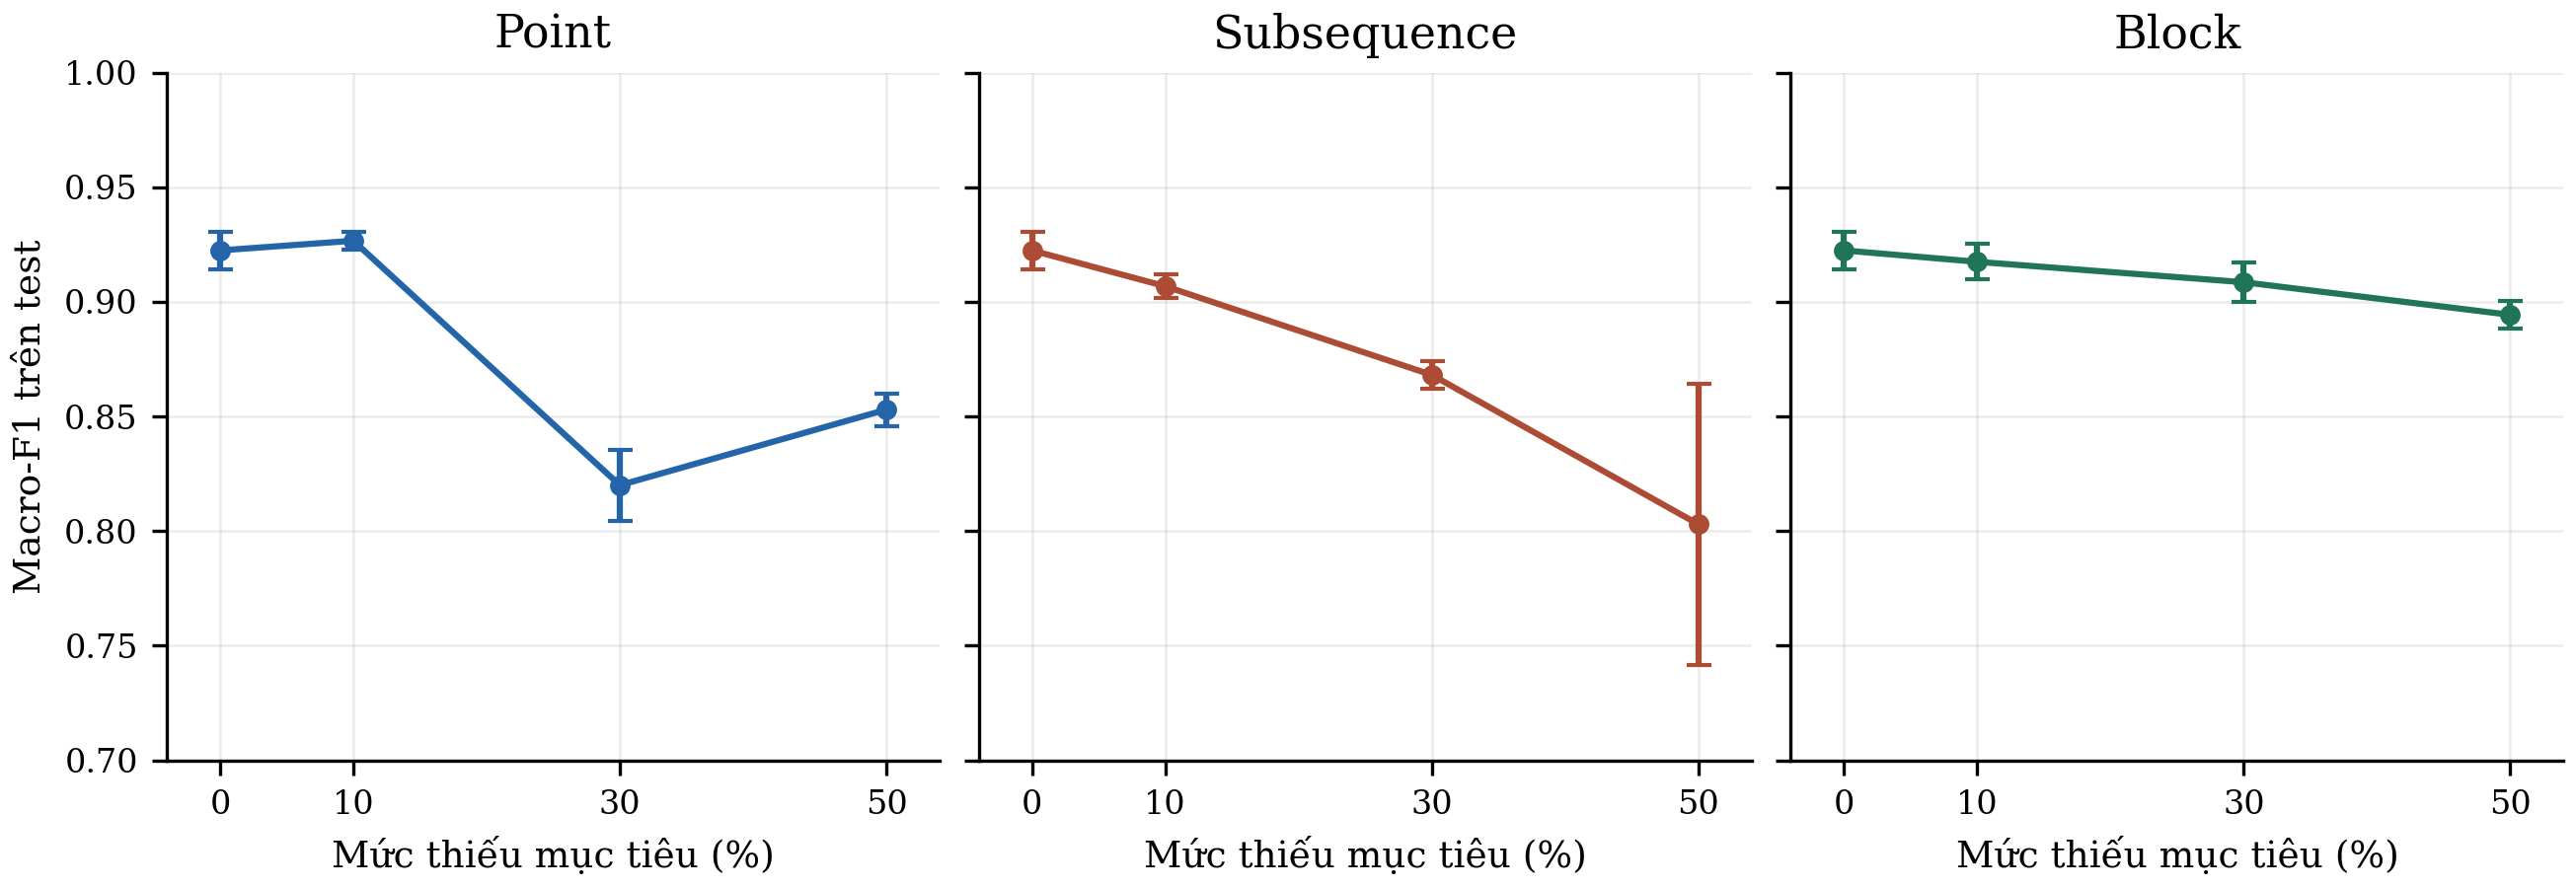
\includegraphics[width=\textwidth]{figs/saits_macro_f1_missingness.png}
\caption{Macro F1 của SAITS theo kiểu và mức thiếu. Điểm là trung bình, thanh
sai số là độ lệch chuẩn mẫu giữa ba seed. Mốc 0\% dùng chung kết quả không ẩn
thêm và vẫn giữ thiếu tự nhiên. Các đường nối chỉ hỗ trợ quan sát xu hướng.}
\label{fig:saits-macro-f1-missingness}
\end{figure}

\paragraph{Ảnh hưởng của mức và kiểu thiếu.}
Không ẩn thêm cho Macro F1 $0.9224 \pm 0.0082$. Ở mức thiếu 50\%, point,
subsequence và block lần lượt đạt $0.8530 \pm 0.0071$, $0.8030 \pm 0.0614$
và $0.8943 \pm 0.0061$, tương ứng giảm khoảng 6.94, 11.94 và 2.81 điểm phần
trăm Macro F1 so với mốc. Trong lần chạy này, block ở mức 30\% và 50\% cho
điểm trung bình cao hơn point/subsequence cùng mức; do đó kết quả SAITS không
ủng hộ nhận định rằng block luôn là kiểu thiếu gây suy giảm mạnh nhất.

\paragraph{Xu hướng không đơn điệu và độ biến thiên giữa seed.}
Point 10\% đạt $0.9266$, nhỉnh hơn mốc không ẩn thêm $0.0042$; point 30\%
đạt $0.8200$, thấp hơn point 50\% ($0.8530$). Vì từng điều kiện được huấn
luyện độc lập, các quan sát này cần được báo cáo nguyên trạng; chưa đủ cơ sở
để kết luận rằng tăng mức thiếu cải thiện mô hình. Subsequence 50\% có độ lệch
chuẩn lớn nhất ($0.0614$): Macro F1 của seed 1, 2 và 42 lần lượt là $0.8411$,
$0.8357$ và $0.7321$ (Phụ lục~\ref{sec:phu-luc-saits-seed}). Sự phân tán này
cho thấy việc báo cáo cả ba seed cần thiết hơn việc chỉ chọn lượt tốt nhất.

\begin{figure}[H]
\centering
\TODO{Vẽ đường suy giảm Macro F1 (và PR-AUC) theo tỷ lệ thiếu dữ liệu (0/10/30/50\%),
mỗi đường ứng với một mô hình, tách thành 3 subplot riêng cho từng kiểu mất dữ liệu
(point/subsequence/block).}
\caption{Suy giảm Macro F1 theo tỷ lệ và kiểu mất dữ liệu.}
\label{fig:suy-giam-macro-f1}
\end{figure}

\TODO{Viết nhận xét định lượng: mô hình nào suy giảm ít nhất ở mỗi kiểu mất dữ liệu, và
liệu kiểu block có gây suy giảm mạnh hơn point/subsequence ở cùng tỷ lệ hay không (dự
kiến có, vì block loại bỏ toàn bộ tín hiệu của một biến trong một khoảng thời gian).}

\subsection{Phân tích theo dải nhiệt độ và theo mùa}
\label{sec:phan-tich-nhiet-do-mua}

\TODO{So sánh Macro F1 của các mô hình riêng trong vùng nhiệt độ chồng lấn 0--4\textdegree C
(Mục~\ref{sec:eda}) so với toàn tập test, và theo từng mùa, để kiểm tra liệu các mô hình
có giữ được lợi thế so với baseline ngưỡng nhiệt độ đúng ở vùng khó nhất hay không.}

\subsection{Ablation}
\label{sec:ablation}

\begin{itemize}
  \item \textbf{Đóng góp của từng nhóm đặc trưng:} so sánh LiteStatTemp đơn lẻ, +catch22,
        +tsfresh, +mask/$\Delta t$, để xác định nhóm đặc trưng đóng góp nhiều nhất.
  \item \textbf{Có/không mask và $\Delta t$:} so sánh cùng một mô hình (ví dụ GRU) với và
        không có hai kênh này, để cô lập đóng góp riêng của thông tin vị trí thiếu.
  \item \textbf{Có/không tuning:} so sánh hiệu năng XGBoost với siêu tham số mặc định so
        với sau khi tuning bằng Optuna (Mục~\ref{sec:tuning-classic-ml}).
  \item \textbf{Xử lý mất cân bằng lớp:} so sánh các chiến lược ở Mục~\ref{sec:mat-can-bang-lop-classic}.
\end{itemize}

\TODO{Trình bày bảng/biểu đồ kết quả ablation và viết nhận xét cho từng dòng trên.}

\subsection{Ý nghĩa thống kê}
\label{sec:y-nghia-thong-ke}

\TODO{Báo cáo kết quả kiểm định McNemar cho các cặp mô hình gần nhau nhất về Macro F1, và
biểu đồ critical difference từ kiểm định Friedman (Mục~\ref{sec:kiem-dinh-thong-ke}), nêu
rõ nhóm mô hình không khác biệt có ý nghĩa thống kê ở mức $\alpha = 0.05$.}

\subsection{Chi phí tính toán}
\label{sec:chi-phi-tinh-toan}

\begin{table}[H]
\centering
\caption{Thời gian huấn luyện/suy luận và kích thước mô hình.}
\label{tab:chi-phi-tinh-toan}
\begin{tabular}{@{}lccc@{}}
\toprule
\textbf{Mô hình} & \textbf{Thời gian huấn luyện} & \textbf{Thời gian suy luận / mẫu} & \textbf{Số tham số} \\
\midrule
\TODO{} & \TODO{} & \TODO{} & \TODO{} \\
\bottomrule
\end{tabular}
\end{table}

\subsection{Giải thích mô hình}
\label{sec:giai-thich-mo-hinh-ket-qua}

\TODO{Trình bày SHAP summary plot cho XGBoost và Integrated Gradients cho mô hình học sâu
tốt nhất, cùng phân tích định tính 2--3 ca dự đoán sai điển hình (ví dụ mẫu có nhiệt độ
trong vùng chồng lấn và tỷ lệ thiếu dữ liệu cao).}

\subsection{Thảo luận}
\label{sec:thao-luan}

\paragraph{Phạm vi kết luận từ thực nghiệm SAITS.}
Các kết quả trên phản ánh khả năng phân loại Rain/Snow của cấu hình SAITS đã
chạy: dữ liệu đầu vào giữ nguyên đơn vị, có mask, tối ưu weighted cross-entropy
và chọn checkpoint theo validation loss. Chưa có ablation có/không chuẩn hóa,
kiểm định khác biệt giữa mô hình, hay đánh giá sai số điền thiếu trong phần
kết quả này. Vì vậy, chưa quy chênh lệch quan sát được cho riêng một thành
phần kiến trúc, chưa kết luận SAITS vượt các baseline, và không dùng Macro F1
để suy ra độ chính xác của các giá trị thời tiết được điền.

\TODO{Trả lời trực tiếp câu hỏi nghiên cứu ở Mục~\ref{sec:cau-hoi-nghien-cuu} dựa trên kết
quả ở trên, so sánh với các phát hiện trong tài liệu (Chương~\ref{sec:tong-quan-tai-lieu}),
và nêu rõ giới hạn của các kết luận (ví dụ chỉ áp dụng cho một trạm quan trắc, nhãn suy ra
từ API).}
